\documentclass[aspectratio=169]{beamer}
\usepackage[utf8]{inputenc}
\usepackage[T1]{fontenc}
\usepackage[spanish,es-nodecimaldot]{babel}
\usepackage{amsfonts,amsmath,amssymb,oldgerm}
\usepackage{graphicx}
\usepackage{booktabs}
\usepackage{array}
\usepackage{url}
\usepackage{tikz}
\usepackage{pgfplots}
\usetikzlibrary{positioning,arrows.meta,calc}
\usetheme{_statale}
\usefonttheme[onlymath]{serif}

\titlebackground*{assets/background}
\title{Práctica 1}
\subtitle{Equipos de RF -- Analizador de espectros}
\course{Circuitos de RF -- 2026-II}
\author{Paola Alejandra Bello Buitrago\\José Miguel Sánchez Vargas\\Ricardo Velásquez Martínez}
\date{Universidad Nacional de Colombia -- Sede Bogotá}

\newcommand{\dBm}{\,\mathrm{dBm}}
\newcommand{\ohm}{\,\Omega}
\newcommand{\img}[2][0.8\textwidth]{\includegraphics[width=#1,height=0.68\textheight,keepaspectratio]{#2}}
\newcommand{\smallnote}[1]{\vspace{0.08cm}{\tiny #1}}

\begin{document}
\maketitle

% ================================================================
\begin{frame}{¿Qué buscamos en esta práctica?}
\begin{columns}[T,onlytextwidth]
\begin{column}{0.56\textwidth}
\textbf{Objetivo}\par\medskip
Comprender el funcionamiento y uso de un analizador de espectros para caracterizar señales de radiofrecuencia en el dominio de la frecuencia.
\medskip
\begin{itemize}
    \item Medir frecuencia, potencia y ancho de banda de señales RF.
    \item Observar una banda de FM comercial.
    \item Analizar los armónicos de una señal cuadrada.
    \item Estudiar experimentalmente el efecto del \textbf{RBW}.
    \item Comparar el analizador con la \textbf{FFT} de un osciloscopio.
\end{itemize}
\end{column}
\begin{column}{0.40\textwidth}
\centering
\begin{tikzpicture}[node distance=0.55cm, every node/.style={font=\small}]
\node[draw,rounded corners,fill=statalegrey,minimum width=3.3cm,minimum height=0.85cm] (rf) {Señal RF};
\node[draw,rounded corners,fill=statalegrey,minimum width=3.3cm,minimum height=0.85cm,below=of rf] (sa) {Analizador de espectros};
\node[draw,rounded corners,fill=statalegrey,minimum width=1.4cm,minimum height=0.65cm,below left=0.5cm and -0.05cm of sa] (f) {Frecuencia};
\node[draw,rounded corners,fill=statalegrey,minimum width=1.4cm,minimum height=0.65cm,below right=0.5cm and -0.05cm of sa] (p) {Potencia};
\draw[-{Latex}] (rf)--(sa);
\draw[-{Latex}] (sa)--(f);
\draw[-{Latex}] (sa)--(p);
\end{tikzpicture}
\end{column}
\end{columns}
\end{frame}

% ================================================================
\begin{frame}{¿Qué es un analizador de espectros?}
\begin{columns}[T,onlytextwidth]
\begin{column}{0.48\textwidth}
Un analizador de espectros permite observar cómo se distribuye la potencia de una señal en función de la frecuencia.
\medskip
\begin{block}{Dominios de representación}
\[
x(t)\quad\longrightarrow\quad X(f)
\]
\centering
Tiempo \hspace{1.4cm} Frecuencia
\end{block}
\medskip
Una señal cuadrada periódica presenta una componente fundamental y armónicos impares:
\[
f_0,\;3f_0,\;5f_0,\;7f_0,\ldots
\]
\end{column}
\begin{column}{0.48\textwidth}
\centering
\begin{tikzpicture}[x=0.75cm,y=0.045cm]
\draw[->] (0,0)--(8,0) node[right]{\scriptsize $f$};
\draw[->] (0,0)--(0,90) node[above]{\scriptsize Amplitud};
\foreach \x/\h in {1/78,3/55,5/42,7/32}{\draw[very thick] (\x,0)--(\x,\h);}
\node[below] at (1,0){\scriptsize $f_0$};
\node[below] at (3,0){\scriptsize $3f_0$};
\node[below] at (5,0){\scriptsize $5f_0$};
\node[below] at (7,0){\scriptsize $7f_0$};
\end{tikzpicture}
\medskip
\begin{alertblock}{Pregunta central}
¿Qué componentes de frecuencia contiene realmente una señal RF?
\end{alertblock}
\end{column}
\end{columns}
\end{frame}

% ================================================================
\begin{frame}{¿Cómo funciona el analizador?}
\centering
\begin{tikzpicture}[node distance=0.65cm, every node/.style={font=\small}, block/.style={draw,rounded corners,minimum width=2.25cm,minimum height=0.95cm,align=center,fill=statalegrey}]
\node[block] (in) {Entrada\\RF};
\node[block,right=of in] (att) {Atenuador\\/ protección};
\node[block,right=of att] (mix) {Mezclador};
\node[block,right=of mix] (if) {Filtro IF\\/ RBW};
\node[block,right=of if] (det) {Detector\\ADC + DSP};
\node[block,right=of det] (out) {Pantalla};
\draw[-{Latex},thick] (in)--(att)--(mix)--(if)--(det)--(out);
\node[above=0.35cm of mix] (lo) {Oscilador local (LO)};
\draw[-{Latex},thick] (lo)--(mix);
\end{tikzpicture}
\vspace{0.35cm}
\begin{columns}[T,onlytextwidth]
\begin{column}{0.31\textwidth}\centering\textbf{Mezclador}\par Traslada la señal de entrada a una frecuencia intermedia.\end{column}
\begin{column}{0.31\textwidth}\centering\textbf{RBW}\par Define la resolución con la que se distinguen componentes cercanas.\end{column}
\begin{column}{0.31\textwidth}\centering\textbf{Barrido}\par El LO cambia de frecuencia para recorrer el intervalo seleccionado.\end{column}
\end{columns}
\smallnote{Arquitectura funcional simplificada de un analizador superheterodino.}
\end{frame}

% ================================================================
\begin{frame}{¿Qué vamos a medir?}
\begin{columns}[T,onlytextwidth]
\begin{column}{0.47\textwidth}
\begin{block}{01 -- Banda FM comercial}
Antena $\rightarrow$ DSA832E $\rightarrow$ identificación de una emisora.
\[
f_c,\qquad P,\qquad BW,\qquad SNR
\]
\end{block}
\end{column}
\begin{column}{0.47\textwidth}
\begin{block}{02 -- Señal cuadrada}
Generador $\rightarrow$ DSA832E.
\[
f_0,\;3f_0,\;5f_0,\;7f_0,\ldots
\]
\centering
\boxed{\text{Efecto del RBW}}
\end{block}
\end{column}
\end{columns}
\vfill
\centering
\textbf{Comparación adicional:} analizador de espectros vs. FFT del osciloscopio.
\end{frame}

% ================================================================
\begin{frame}{3. Trabajo previo -- Unidades y potencia}
En RF es común expresar la potencia en \textbf{dBm}:
\[
\boxed{P_{\mathrm{dBm}}=10\log_{10}\left(\frac{P}{1\,\mathrm{mW}}\right)}
\]
\[
P_{\mathrm{mW}}=10^{P_{\mathrm{dBm}}/10}
\]
\begin{columns}[T,onlytextwidth]
\begin{column}{0.42\textwidth}
\begin{block}{Referencias}
\begin{center}
\begin{tabular}{cc}
\toprule
Potencia & dBm\\
\midrule
$1\,mW$ & $0\dBm$\\
$10\,mW$ & $10\dBm$\\
$100\,mW$ & $20\dBm$\\
\bottomrule
\end{tabular}
\end{center}
\end{block}
\end{column}
\begin{column}{0.52\textwidth}
Para una carga resistiva:
\[
\boxed{P=\frac{V_{\mathrm{rms}}^2}{R}}
\]
La impedancia de la carga debe considerarse al relacionar potencia y tensión.
\end{column}
\end{columns}
\end{frame}

% ================================================================
\begin{frame}{Trabajo previo -- Cálculo 1}
\textbf{¿Qué potencia corresponde a $-15\dBm$ sobre $50\,\Omega$?}
\[
P=10^{-15/10}\,mW=0.0316\,mW=31.6\,\mu W
\]
\[
V_{\mathrm{rms}}=\sqrt{PR}
=\sqrt{31.6\times10^{-6}\cdot50}
\]
\begin{center}
\boxed{V_{\mathrm{rms}}\approx39.8\,mV}
\end{center}
\vfill
\centering
\boxed{-15\dBm\;\longrightarrow\;31.6\,\mu W\;\longrightarrow\;39.8\,mV_{\mathrm{rms}}}
\end{frame}

% ================================================================
\begin{frame}{Trabajo previo -- Cálculo 2}
\textbf{¿Qué potencia en dBm corresponde a $0.2\,V_{\mathrm{rms}}$ sobre $75\,\Omega$?}
\[
P=\frac{(0.2)^2}{75}=0.533\,mW
\]
\[
P_{\mathrm{dBm}}=10\log_{10}(0.533)
\]
\begin{center}
\boxed{P_{\mathrm{dBm}}\approx-2.73\,dBm}
\end{center}
\vfill
\centering
\textbf{Resultado:} $0.2\,V_{\mathrm{rms}}$ sobre $75\,\Omega$ equivale a aproximadamente $-2.73\dBm$.
\end{frame}

% ================================================================
\begin{frame}{Trabajo previo -- Cálculo 3}
\textbf{Amplificador: $R_{in}=70\,\Omega$, $R_{out}=40\,\Omega$}
\begin{columns}[T,onlytextwidth]
\begin{column}{0.47\textwidth}
\begin{block}{Entrada}
$V_{in}=1\,mV_{rms}$
\[
P_{in}=\frac{(1mV)^2}{70}
\]
\[
\boxed{P_{in}\approx-48.45\dBm}
\]
\end{block}
\end{column}
\begin{column}{0.47\textwidth}
\begin{block}{Salida}
$V_{out}=2\,mV_{rms}$
\[
P_{out}=\frac{(2mV)^2}{40}
\]
\[
\boxed{P_{out}=-40\dBm}
\]
\end{block}
\end{column}
\end{columns}
\begin{center}
\boxed{G_{P,dB}=P_{out,dBm}-P_{in,dBm}\approx8.45\,dB}
\end{center}
\end{frame}

% ================================================================
\begin{frame}{Trabajo previo -- Cálculo 4}
\textbf{Potencia de $-5\dBm$ sobre una carga de $500\,\Omega$}
\[
P=10^{-5/10}\,mW=0.316\,mW=3.16\times10^{-4}\,W
\]
\[
V_{\mathrm{rms}}=\sqrt{PR}
=\sqrt{3.16\times10^{-4}\cdot500}
\]
\begin{center}
\boxed{V_{\mathrm{rms}}\approx397.6\,mV}
\end{center}
\vfill
\centering
La sonda se considera ideal: no carga el circuito.
\end{frame}

% ================================================================
\begin{frame}{3.2 -- El analizador de espectros: RIGOL DSA832E}
\begin{columns}[T,onlytextwidth]
\begin{column}{0.48\textwidth}
\centering
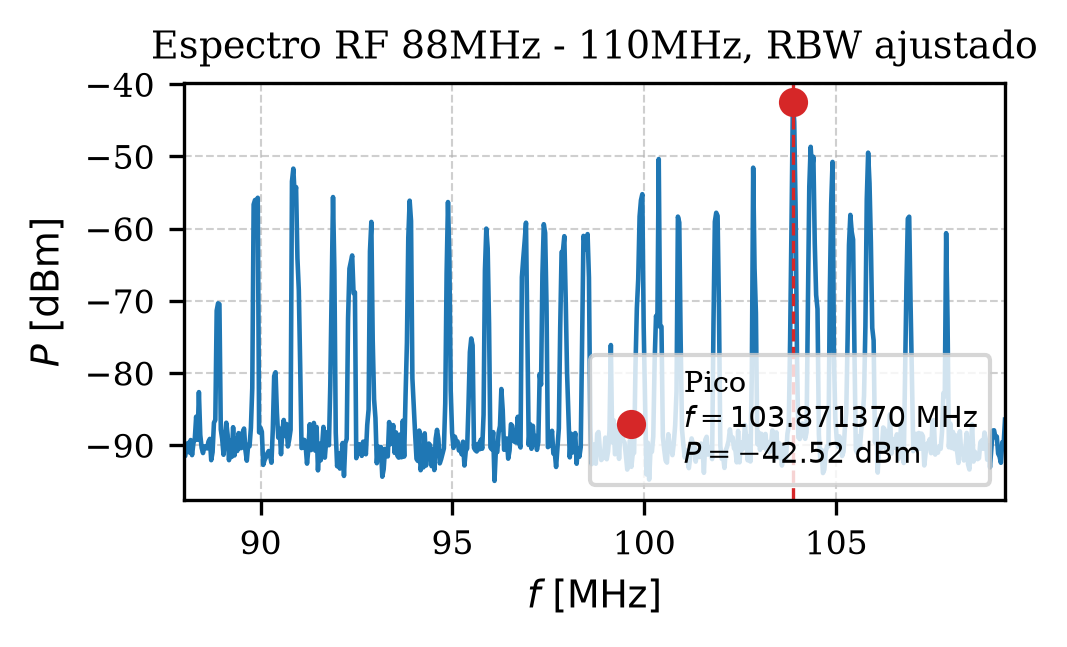
\includegraphics[width=0.95\textwidth,height=0.53\textheight,keepaspectratio]{imgs/rf/rf_medida_1_2.png}
\end{column}
\begin{column}{0.48\textwidth}
\textbf{Características a identificar en la práctica:}
\begin{itemize}
    \item Tipo de conector de entrada.
    \item Rango de frecuencias.
    \item Span.
    \item Tiempo de barrido.
    \item Rango de amplitudes.
    \item Nivel máximo de entrada.
    \item RBW y VBW.
    \item Impedancia de entrada.
\end{itemize}
\end{column}
\end{columns}
\smallnote{Equipo principal empleado durante la práctica.}
\end{frame}

% ================================================================
\begin{frame}{Parámetros que controlan la medición}
\begin{columns}[T,onlytextwidth]
\begin{column}{0.48\textwidth}
\begin{block}{Frecuencia}
\[
\boxed{\text{Center Frequency + Span}}
\]
Define la zona del espectro observada.
\end{block}
\begin{block}{Resolución}
\[
\boxed{RBW}
\]
Determina qué tan próximas pueden estar dos componentes para distinguirse.
\end{block}
\end{column}
\begin{column}{0.48\textwidth}
\begin{block}{Barrido}
\[
\boxed{\text{Sweep Time}}
\]
Tiempo necesario para recorrer el intervalo seleccionado.
\end{block}
\begin{block}{Nivel}
\[
\boxed{\text{Reference Level}}
\]
Define la escala vertical de amplitud.
\end{block}
\end{column}
\end{columns}
\centering
\small RBW menor $\Rightarrow$ mayor resolución espectral y, en general, mayor tiempo de barrido.
\end{frame}

% ================================================================
\begin{frame}{Comparación de los analizadores y conexiones}
\begin{columns}[T,onlytextwidth]
\begin{column}{0.55\textwidth}
\begin{tabular}{p{0.27\textwidth}p{0.62\textwidth}}
\toprule
\textbf{Equipo} & \textbf{Aplicación en la práctica}\\
\midrule
RIGOL DSA832E & Análisis de señales RF en laboratorio.\\
RIGOL FSW43 & Análisis RF/microondas de mayor desempeño.\\
RF Explorer & Exploración portátil del espectro.\\
\bottomrule
\end{tabular}
\medskip
\begin{center}
\small Frecuencia + sensibilidad + resolución + portabilidad + funciones
\end{center}
\end{column}
\begin{column}{0.40\textwidth}
\begin{alertblock}{Conexión RF}
Antes de medir:
\[
\boxed{\text{Conector}\rightarrow\text{Adaptador}\rightarrow50\,\Omega}
\]
Verificar conectores, adaptadores y la impedancia de referencia.
\end{alertblock}
\end{column}
\end{columns}
\end{frame}

% ================================================================
\begin{frame}{4.1 -- Visualización de una banda FM comercial}
\begin{columns}[T,onlytextwidth]
\begin{column}{0.58\textwidth}
\centering
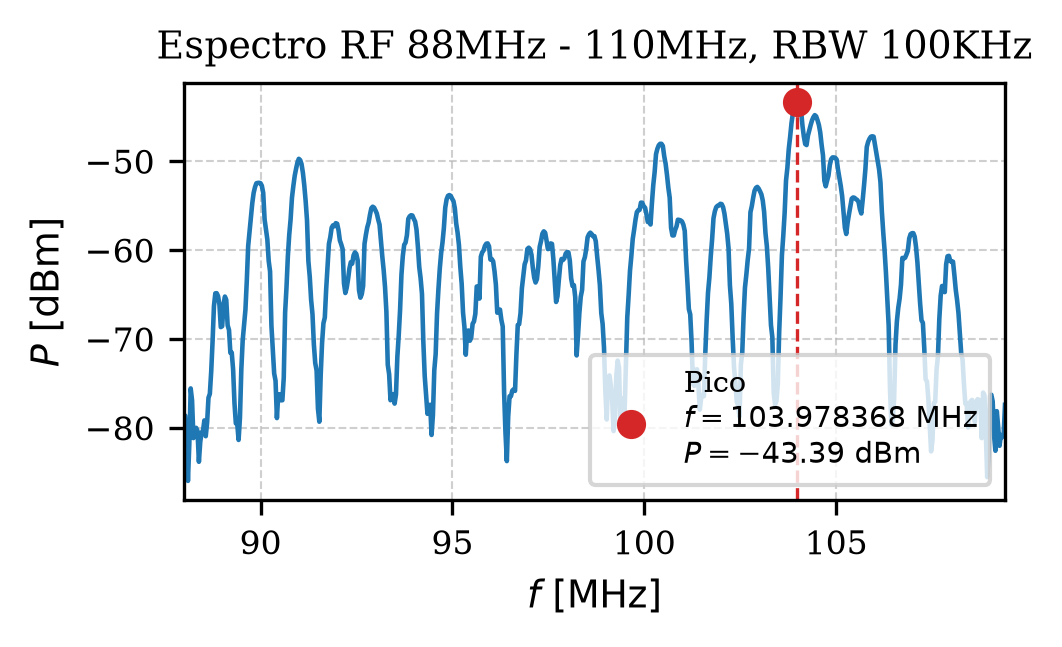
\includegraphics[width=\textwidth,height=0.64\textheight,keepaspectratio]{imgs/rf/rf_medida_1_1.png}
\end{column}
\begin{column}{0.38\textwidth}
\textbf{Montaje}\par
Antena $\rightarrow$ DSA832E
\medskip

\textbf{Objetivo}\par
Observar la banda comercial de FM e identificar la emisora con mayor nivel de potencia recibido.
\medskip

\textbf{Caracterización}\par
\[
f_c,\qquad P,\qquad BW,\qquad SNR
\]
\small
Identificar además el nombre comercial del operador.
\end{column}
\end{columns}
\end{frame}

% ================================================================
\begin{frame}{4.1 -- RBW, tiempo de barrido y relación señal/ruido}
\begin{columns}[T,onlytextwidth]
\begin{column}{0.52\textwidth}
\centering
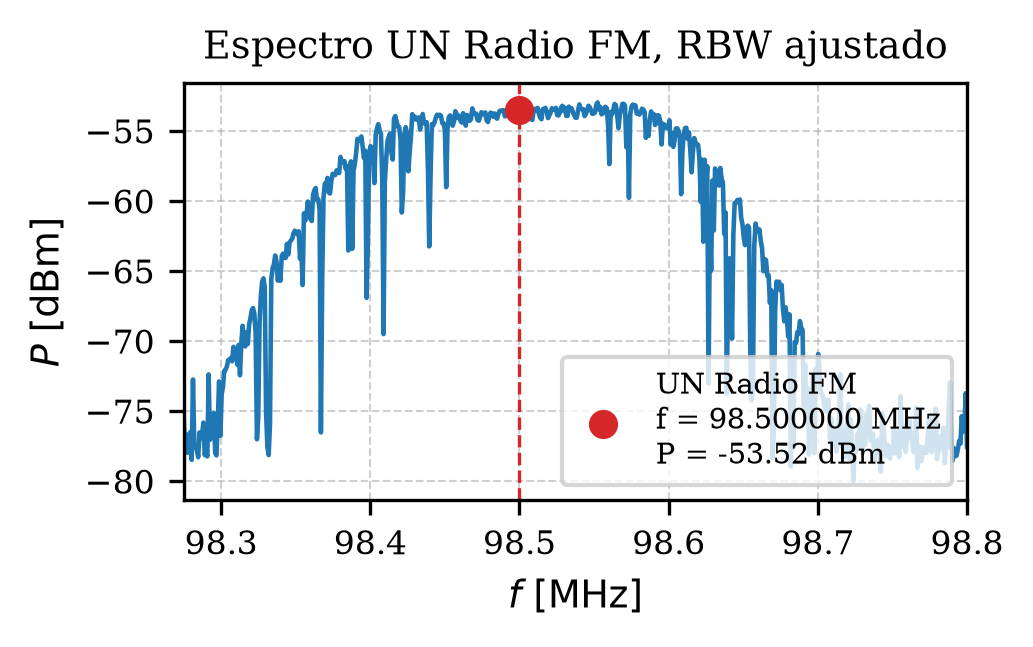
\includegraphics[width=\textwidth,height=0.62\textheight,keepaspectratio]{imgs/rf/rf_medida_1_4.png}
\end{column}
\begin{column}{0.43\textwidth}
\textbf{Relación experimental}\par\medskip
\[
RBW\downarrow
\quad\Rightarrow\quad
\text{resolución}\uparrow
\quad\Rightarrow\quad
\text{Sweep Time}\uparrow
\]
\medskip
\textbf{Optimización}\par
Modificar la configuración hasta obtener la mejor relación señal/ruido y documentar el valor logrado.
\medskip
\begin{block}{Parámetros a observar}
RBW, VBW, Span, Reference Level y detector.
\end{block}
\end{column}
\end{columns}
\end{frame}

% ================================================================
\begin{frame}{4.2 -- Espectro de una señal cuadrada: mediciones}
\centering
\begin{columns}[T,onlytextwidth]
\begin{column}{0.32\textwidth}\centering
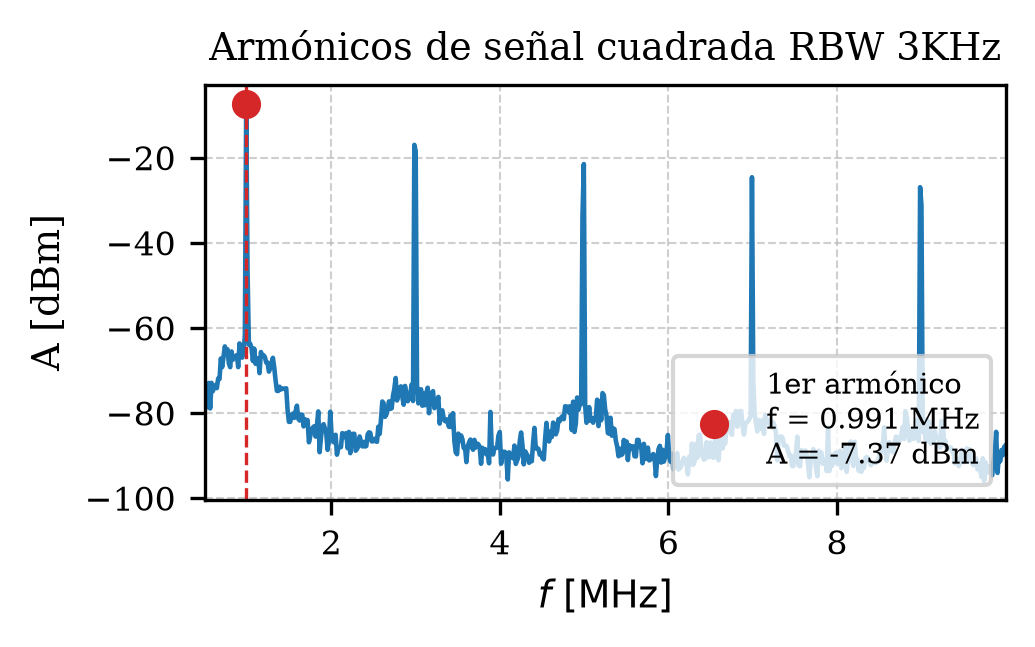
\includegraphics[width=\textwidth,height=0.27\textheight,keepaspectratio]{imgs/rf/armonicos_3_1_db.png}\\[-1mm]
\scriptsize RBW = 3 kHz
\end{column}
\begin{column}{0.32\textwidth}\centering
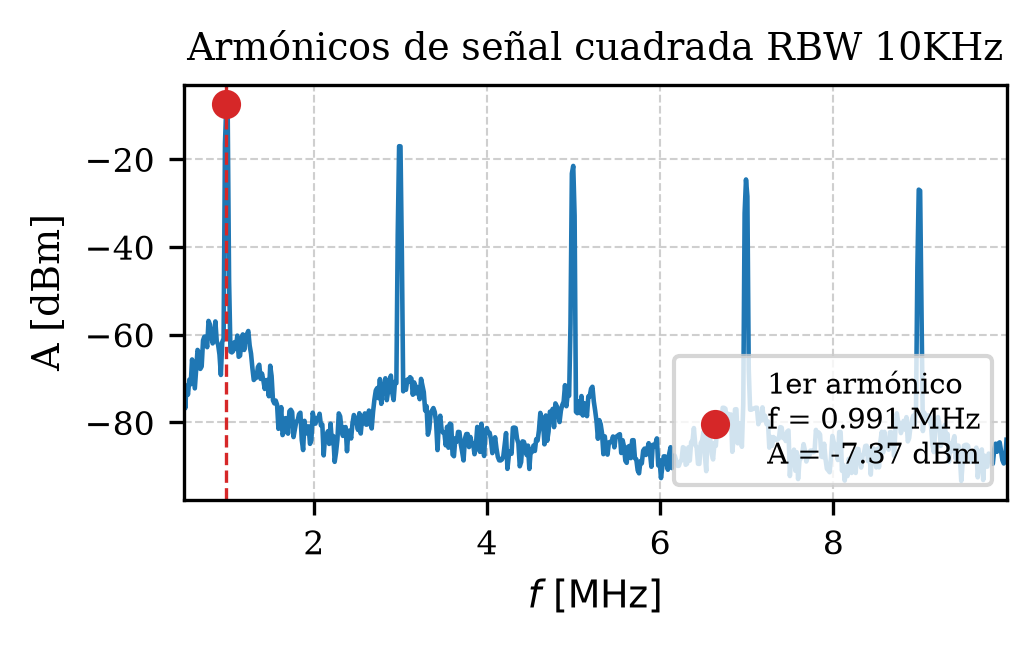
\includegraphics[width=\textwidth,height=0.27\textheight,keepaspectratio]{imgs/rf/armonicos_3_2_db.png}\\[-1mm]
\scriptsize RBW = 10 kHz
\end{column}
\begin{column}{0.32\textwidth}\centering
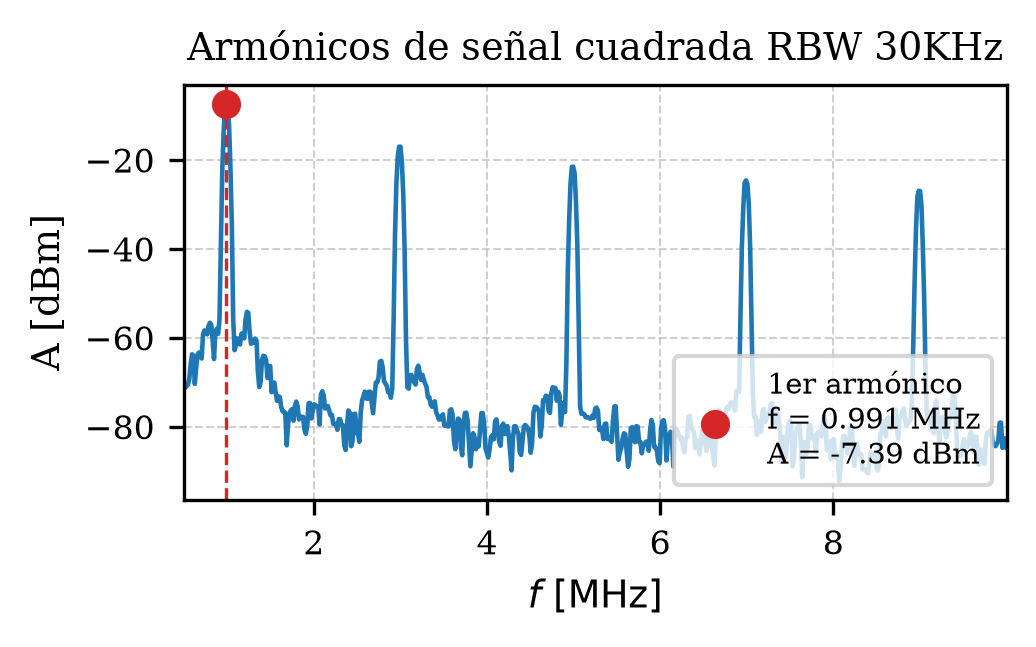
\includegraphics[width=\textwidth,height=0.27\textheight,keepaspectratio]{imgs/rf/armonicos_3_3_db.png}\\[-1mm]
\scriptsize RBW = 30 kHz
\end{column}
\end{columns}
\vspace{0.12cm}
\begin{columns}[T,onlytextwidth]
\begin{column}{0.32\textwidth}\centering
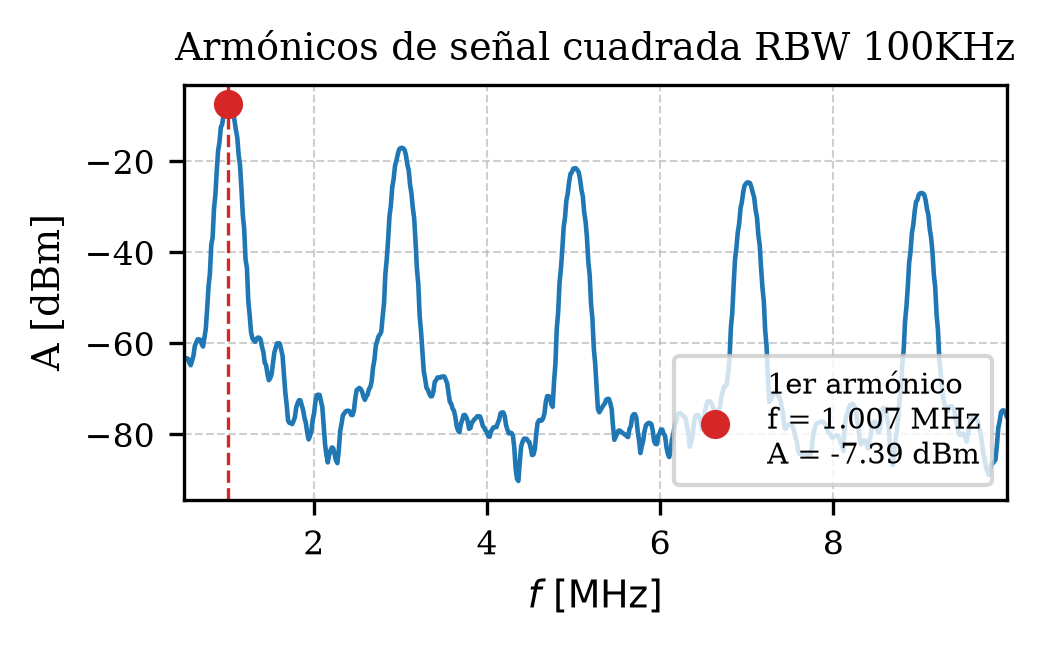
\includegraphics[width=\textwidth,height=0.27\textheight,keepaspectratio]{imgs/rf/armonicos_3_4_db.png}\\[-1mm]
\scriptsize RBW = 100 kHz
\end{column}
\begin{column}{0.32\textwidth}\centering
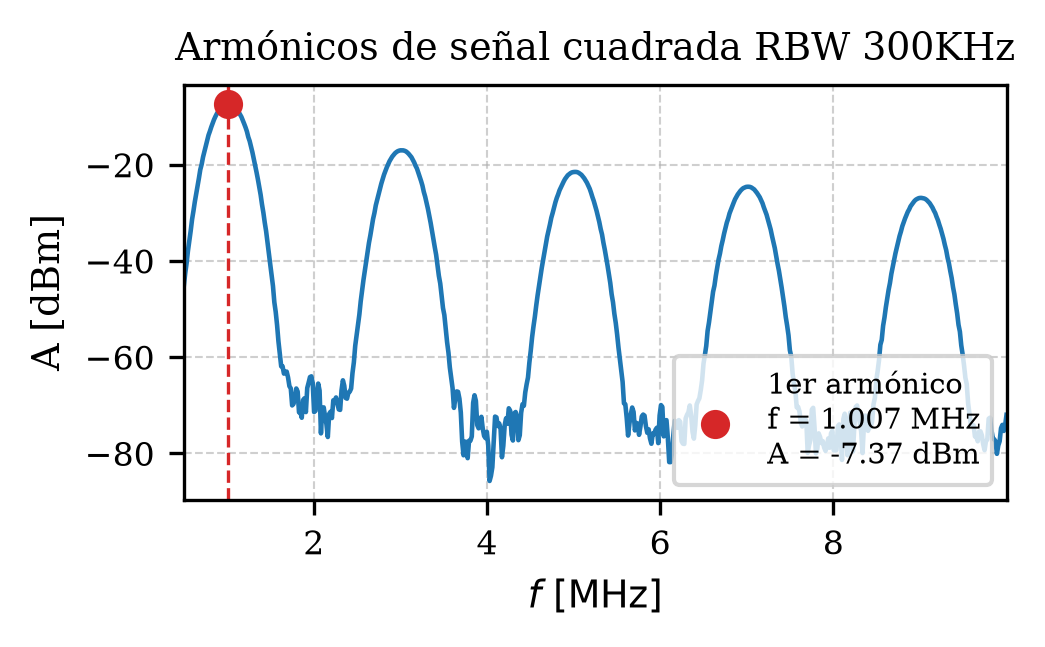
\includegraphics[width=\textwidth,height=0.27\textheight,keepaspectratio]{imgs/rf/armonicos_3_5_db.png}\\[-1mm]
\scriptsize RBW = 300 kHz
\end{column}
\begin{column}{0.32\textwidth}\centering
\textbf{Medición}\par\medskip
Cinco armónicos de la señal cuadrada y comparación para cinco valores de RBW.
\end{column}
\end{columns}
\end{frame}

% ================================================================
\begin{frame}{4.2 -- Preguntas y respuestas experimentales}
\begin{columns}[T,onlytextwidth]
\begin{column}{0.47\textwidth}
\textbf{Preguntas de la guía}
\begin{enumerate}
    \item ¿Cuál es el RBW fijado automáticamente por el analizador?
    \item ¿Qué diferencias aparecen al variar el RBW entre 3 kHz y 300 kHz?
    \item ¿Cuál es el efecto del RBW sobre la señal visualizada?
    \item ¿Qué diferencias existen frente a la FFT del osciloscopio?
    \item ¿Cuáles son las posibles causas de esas diferencias?
\end{enumerate}
\end{column}
\begin{column}{0.50\textwidth}
\centering
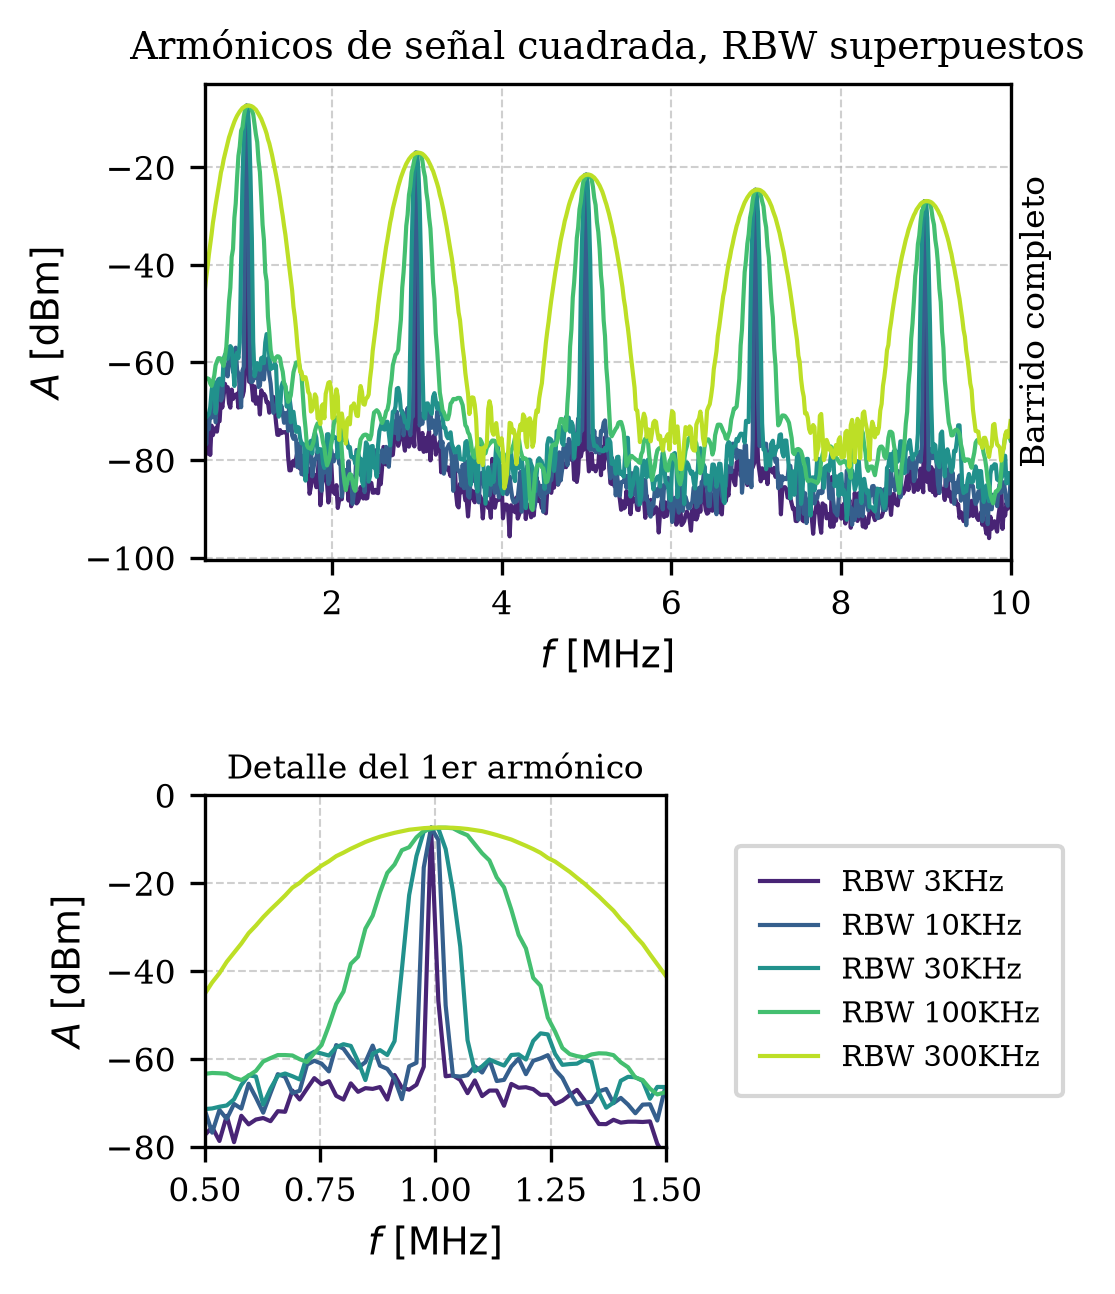
\includegraphics[width=\textwidth,height=0.56\textheight,keepaspectratio]{imgs/rf/armonicos_3_superpuestos.png}
\end{column}
\end{columns}
\vspace{-0.1cm}
\scriptsize
\textbf{Respuesta sintetizada:} al reducir el RBW se mejora la resolución espectral y se distinguen mejor componentes cercanas, a costa de un mayor tiempo de barrido. La FFT depende además de la frecuencia de muestreo, longitud de registro y ventana empleada.
\end{frame}

% ================================================================
\begin{frame}{Comparación: analizador de espectros vs. FFT}
\begin{columns}[T,onlytextwidth]
\begin{column}{0.49\textwidth}
\centering
\textbf{DSA832E}\par
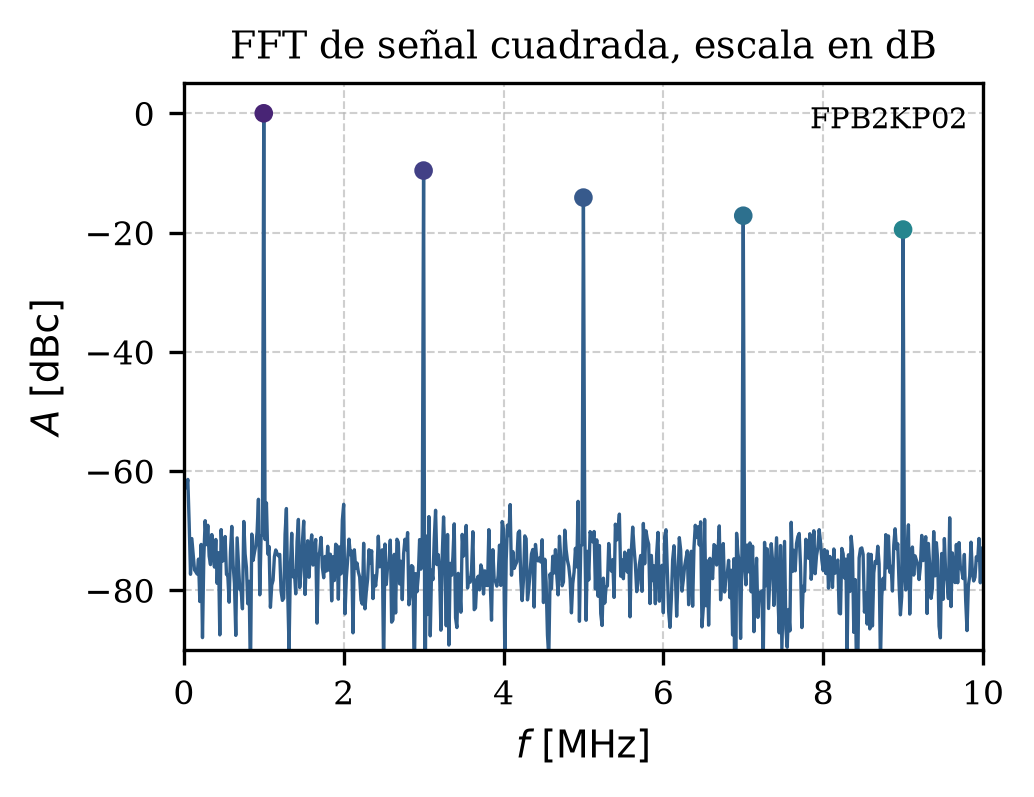
\includegraphics[width=\textwidth,height=0.55\textheight,keepaspectratio]{imgs/rf/fft_5_1_db.png}
\end{column}
\begin{column}{0.49\textwidth}
\centering
\textbf{FFT del osciloscopio}\par
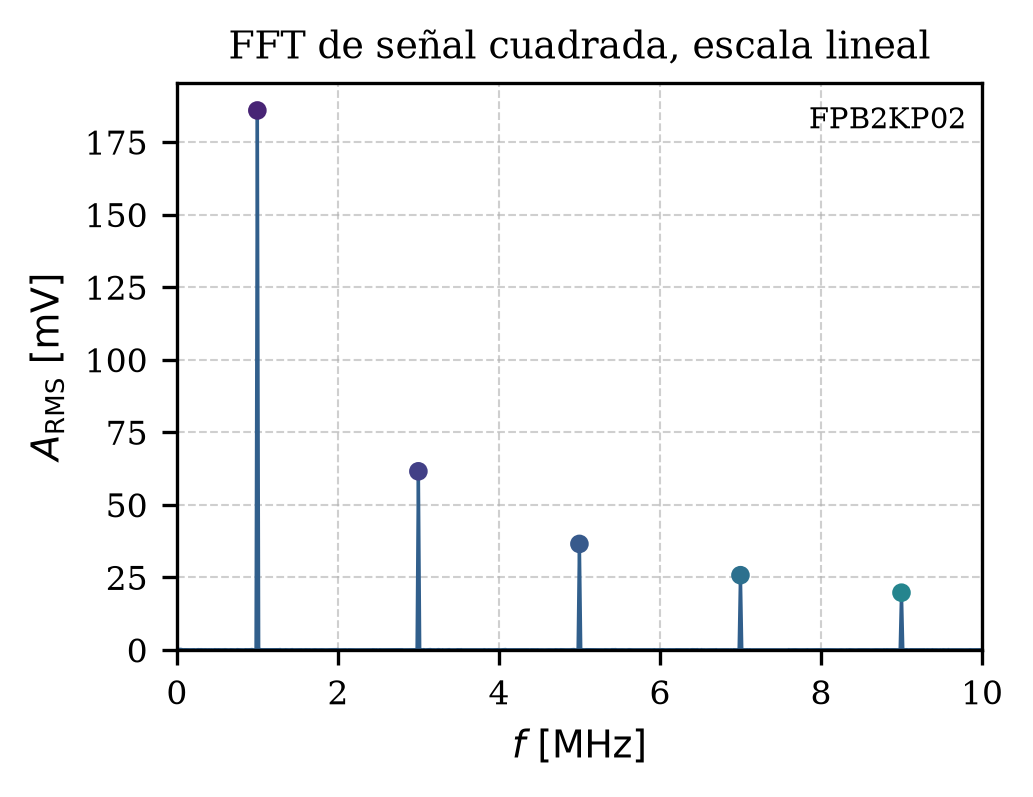
\includegraphics[width=\textwidth,height=0.55\textheight,keepaspectratio]{imgs/rf/fft_5_2_lineal.png}
\end{column}
\end{columns}
\small
Las diferencias pueden asociarse al método de adquisición, resolución, ventana de FFT, tiempo de observación, escalas y piso de ruido.
\end{frame}

% ================================================================
\begin{frame}{Conclusiones}
\begin{enumerate}
    \item El analizador de espectros permite caracterizar señales RF en el dominio de la frecuencia mediante frecuencia, potencia y ancho de banda.
    \item El \textbf{RBW} establece un compromiso entre resolución espectral y tiempo de barrido.
    \item La señal cuadrada permitió observar experimentalmente sus \textbf{armónicos impares} y estudiar el efecto de la resolución.
    \item La comparación con la FFT mostró que dos métodos de análisis pueden presentar diferencias por sus condiciones de adquisición y procesamiento.
\end{enumerate}
\vfill
\centering
\Large\textbf{La configuración del instrumento es parte de la medición.}
\end{frame}

\backmatter
\end{document}
